\documentclass[column]{article}

\usepackage{graphicx} % Per includere immagini
\usepackage{amsmath}  % Per formule matematiche avanzate
\usepackage{amssymb}  % Per simboli matematici aggiuntivi
\usepackage{hyperref} % Per hyperlink nel documento
\usepackage{multicol} % Per gestire le colonne
\usepackage{hyperref}
\usepackage{booktabs}
\usepackage[left=3cm,right=3cm]{geometry}



% Informazioni sul documento
\title{Self-Supervised Learning for Endoscopic Video Analysis - PyTorch implementation}
\author{Cordioli Davide - VR510529}

\begin{document}
	
	\maketitle
	
	\begin{multicols}{2}
		
	\section{Introduction}
	
	PyTorch is probably the most used framework for developing artificial intelligence applications, thanks to its intuitive approach. In this project it has been studied the code that can be found in the GitHub repository  \href{https://github.com/royhirsch/endossl}{RoyHirsch / endossl}, which has been written using TensorFlow, with the objective of replicating it using PyTorch.
	
	The code is referred to the paper \textit{Self-Supervised Learning for Endoscopic Video Analysis} [1], where is described how the Masked Siamese Networks (MSN), a technique for Self Supervised Learning (SSL), can be applied to endoscopic video. MSN, that will be explained better latter on, allow us to build a model capable of extracting the most relevant features from the image, features that can be then used for tasks like frame classifications.
	
	\section{Objective}
	
	As the original paper has reported, the applications of MSN, done on 7 TPU, required a total of 800 epochs of training for the smallest model, with a batch size of 1024. The authors of the original code had uploaded the pre-trained model in JAX, but the conversion in PyTorch was not possible. So, at the beginning it has been used another pre-trained model, trained using ImageNet-1K, which could have been used with PyTorch, but the classification converged to very poor results. 
	
	For this reason it has been decided to develop the MSN training procedure, which execution was not executed as the paper described since our devices are not such powerful as 7 TPU, but it has been reproduced over a few epochs, with reduced batch size, in order to show the convergence of MSN technique over Cholec80 dataset.
	
	
	\section{Masked Siamese Networks}
	In this section, is shortly described the MSN technique, all the mathematics part are omitted for avoiding this report to become too long, but the reader can see all the details in the paper \textit{Masked Siamese Networks for Label-Efficient Learning}[2]. The structure of the process used by the MSN is described in figure 1. 
	
	During the training, to an image are applied some random data augmentations, obtaining and anchor and a target view, different versions of same image. Then is applied a patch over both target and anchor views, but on the anchor view is also applied a random masking for removing some of the patches. 
	
	Then, both the images are given in input to $f_\theta$ and $f_{\overline{\theta}}$: two feature extractor that must share the same structure. For this project, two \textit{visual transformers} has been used. Then the output of the the feature extractors, $z$ for anchor view and $z^+$ for target view, are then compared to a learnable set $\bf q \in \mathbb{R}^{K \times d}$ of $K$ prototypes of dimension $d$, where $d$ is also the dimension of the latent space, following the formula
	
	\begin{equation}
		p_{i} := \textnormal{softmax}\left(\frac{z_i \cdot \bf q}{\tau}\right)
	\end{equation}
	
	where $i$ indicates the $i$-th element in the batch and where $\tau\in(0,1)$ is a temperature. So, for both anchor and target view, following (1), it is generated a prediction $p_i$ and $p_i^+$ respectively, used for cluster assignments.
	
	The objective is to minimize the difference between this two predictions, difference measured by a loss function $H(p^+, p)$, usually the cross-entropy. The back-propagation part is applied only over the prototypes and $f_\theta$ with respect of anchor predictions $p_i$, while the weights of $f_{\overline{\theta}}$ are updated using \textit{exponential moving average} over the $f_\theta$ weights. 
	
	It has been also incorporated the \textit{mean entropy maximization} (ME-MAX) regularizer in the loss computation,  to encourage the model to utilize the full set of prototypes.
	
	\end{multicols}
	
	
	\begin{figure}[h]
		\centering
		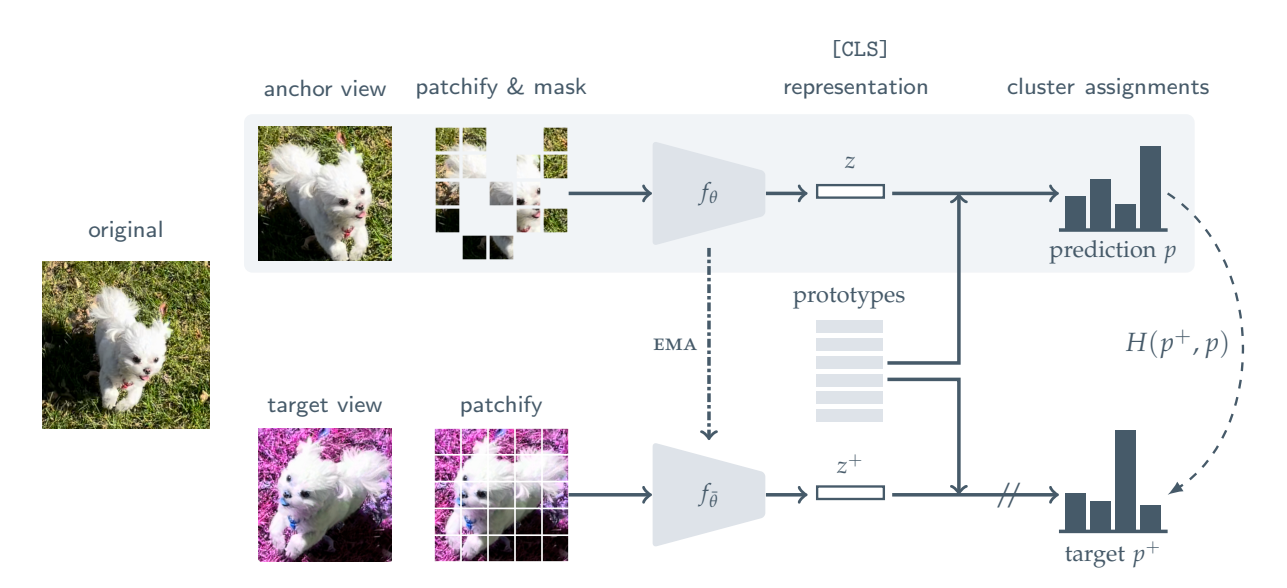
\includegraphics[width=\textwidth]{Images/screenshot001}
		\caption[MSN workflow]{}
		\label{fig:screenshot001}
	\end{figure}
	
	\begin{multicols}{2}
		
		
	\section{Implementation details}
	
	The structure of this project uses PyTorch but also the python module \textit{Transformers}, a library that implement in both TensorFlow and PyTorch some of the most famous deep learning models, including also
	the ViT MSN described above. It allow also to download some pre-trained models, of which the most popular for our porpuses are \textit{facebook/vit-msn-small}, \textit{facebook/vit-msn-base}, \textit{facebook/vit-msn-large}. For the limitations of the architecture used for this project it has been used \textit{facebook/vit-msn-small}, the hyper-parametrs of each model are described in table 1.
	
	During the pre-training part, the number of learnable prototypes is set to 1024, as indicated in the original paper, and the masked part is applied random, masking the 50\% of the patches. Our model can have in input an image of dimension 224 by 224, each patch has a dimension of $16px \times 16px$, so at the end each image will be divided in 196 patches, of which half will be masked in the anchor view.
		
	\end{multicols}
	
	\begin{table}[ht]
			\centering
			\resizebox{\textwidth}{!}{%
			\begin{tabular}{|l|c|c|c|c|c|}
				\hline
				\textbf{Model} & \textbf{Hidden Layers} & \textbf{Hidden dim size} & \textbf{Num heads}
				& \textbf{Num params} & MLP size \\
				\hline
				ViT-Small & 12 & 384 & 6 & 22M & 1536\\
				\hline
				ViT-Base & 12 & 768 & 12 & 86M & 3072\\
				\hline
				ViT-Large & 24 & 1024 & 16 & 307M & 4096\\
				\hline
		\end{tabular}%
		}
		\caption{ViT. models hyper-parameters}
		\label{tab:vit_specs}
	\end{table}
	
		
	\begin{multicols}{2}
		
	\section{Experiments}
	
	The experiment conducted over the Cholec80 datasets for a total of 30 epochs using a batch size of 150. The loss computed is the cross entropy that it has been shown to converge to a value of 5.93, that despite its high value, over a probability vector of 1024 element is very low. 
	
	\section{Conclusion}
	
	Probably a way for improving the results can be for sure using bigger models and training over a higher number of epochs, since the results described in the above section could represent a shoulder point that after more epochs would have been surpassed.
		
	\end{multicols}
	
	
	

	
	\begin{thebibliography}{9}
		
		\bibitem{example1}
		Roy Hirsch, Mathilde Caron, Regev Cohen, Amir Livne, Ron Shapiro, Tomer Golany, Roman Goldenberg, Daniel Freedman, and Ehud Rivlin: Self-Supervised Learning for Endoscopic Video Analysis (2023)
		
		\bibitem{example2}
		Mahmoud Assran, Mathilde Caron, Ishan Misra, Piotr Bojanowski, Florian Bordes, Pascal Vincent, Armand Joulin,  Michael Rabbat, Nicolas Ballas: Masked Siamese Networks for Label-Efficient Learning (2022)
		
	\end{thebibliography}
	
\end{document}